\chapter{Supplementary Information to \Chapref{heterogeneouslandscapes}}


\renewcommand{\thetable}{C.\arabic{table}}
\setcounter{table}{0}

%<><><><><><><><><><><><><><><><><><><><><><><><><><><><><><><><><><><><><><><><><><><><><><><><>
\begin{table}[h]
\centering \small
\caption[Per locus effect size differences]{Per locus effect size differences across scenarios of genetic architecture regimes. The range from minimum to maximum is shown for each scenario, as well as the mean.}
\label{tab:effects}
\begin{tabular}{ccc}
Genetic architecture	&	$\Delta z_{opt}$	&	Per locus difference: range (mean)  \\ \hline \hline
$\mu = 10^{-2}$	& $5$		& $-0.0674 - 0.4603 ~ (0.0190)$	\\ 
$\alpha^2 = 0.005$	& $7.5$		& $-0.0993 - 0.4884 ~ (0.0321)$	\\ 
				& $10$		& $-0.3633 - 0.5311 ~ (0.0479)$	\\ 
				& $12.5$		& $-0.4187 - 0.5464 ~ (0.0583)$	\\ \hline
$\mu = 10^{-3}$	& $5$		& $-0.0655 - 0.2864 ~ (0.0103)$	\\ 
$\alpha^2 = 0.05$	& $7.5$		& $-0.1233 - 0.7258 ~ (0.0277)$	\\ 
				& $10$		& $-0.4088 - 0.8786 ~ (0.0447)$	\\ 
				& $12.5$		& $-0.4308 - 0.6513 ~ (0.0596)$	\\ \hline
$\mu = 10^{-4}$	& $5$		& $-0.0144 - 1.1386 ~ (0.01799)$	\\ 
$\alpha^2 = 0.5$	& $7.5$		& $-0.2206 - 2.6775 ~ (0.0251)$	\\ 
				& $10$		& No expansion	\\ 
				& $12.5$		& No expansion	\\ \hline
$\mu = 10^{-5}$	& $5$		& ${-0.0055} - 2.6881 ~ (0.0228)$	\\ 
$\alpha^2 = 5.0$	& $7.5$		& $-0.1967 - 4.8746 ~ (0.0190)$	\\ 
				& $10$		& $-0.6236 - 6.4207 ~ (0.0522)$	\\ 
				& $12.5$		& No expansion	\\ \hline
\end{tabular}
\end{table}
%<><><><><><><><><><><><><><><><><><><><><><><><><><><><><><><><><><><><><><><><><><><><><><><><>



\renewcommand{\thefigure}{C.\arabic{figure}}
\setcounter{figure}{0}




\begin{figure}[!h]
\centering
\makebox[\textwidth]{
        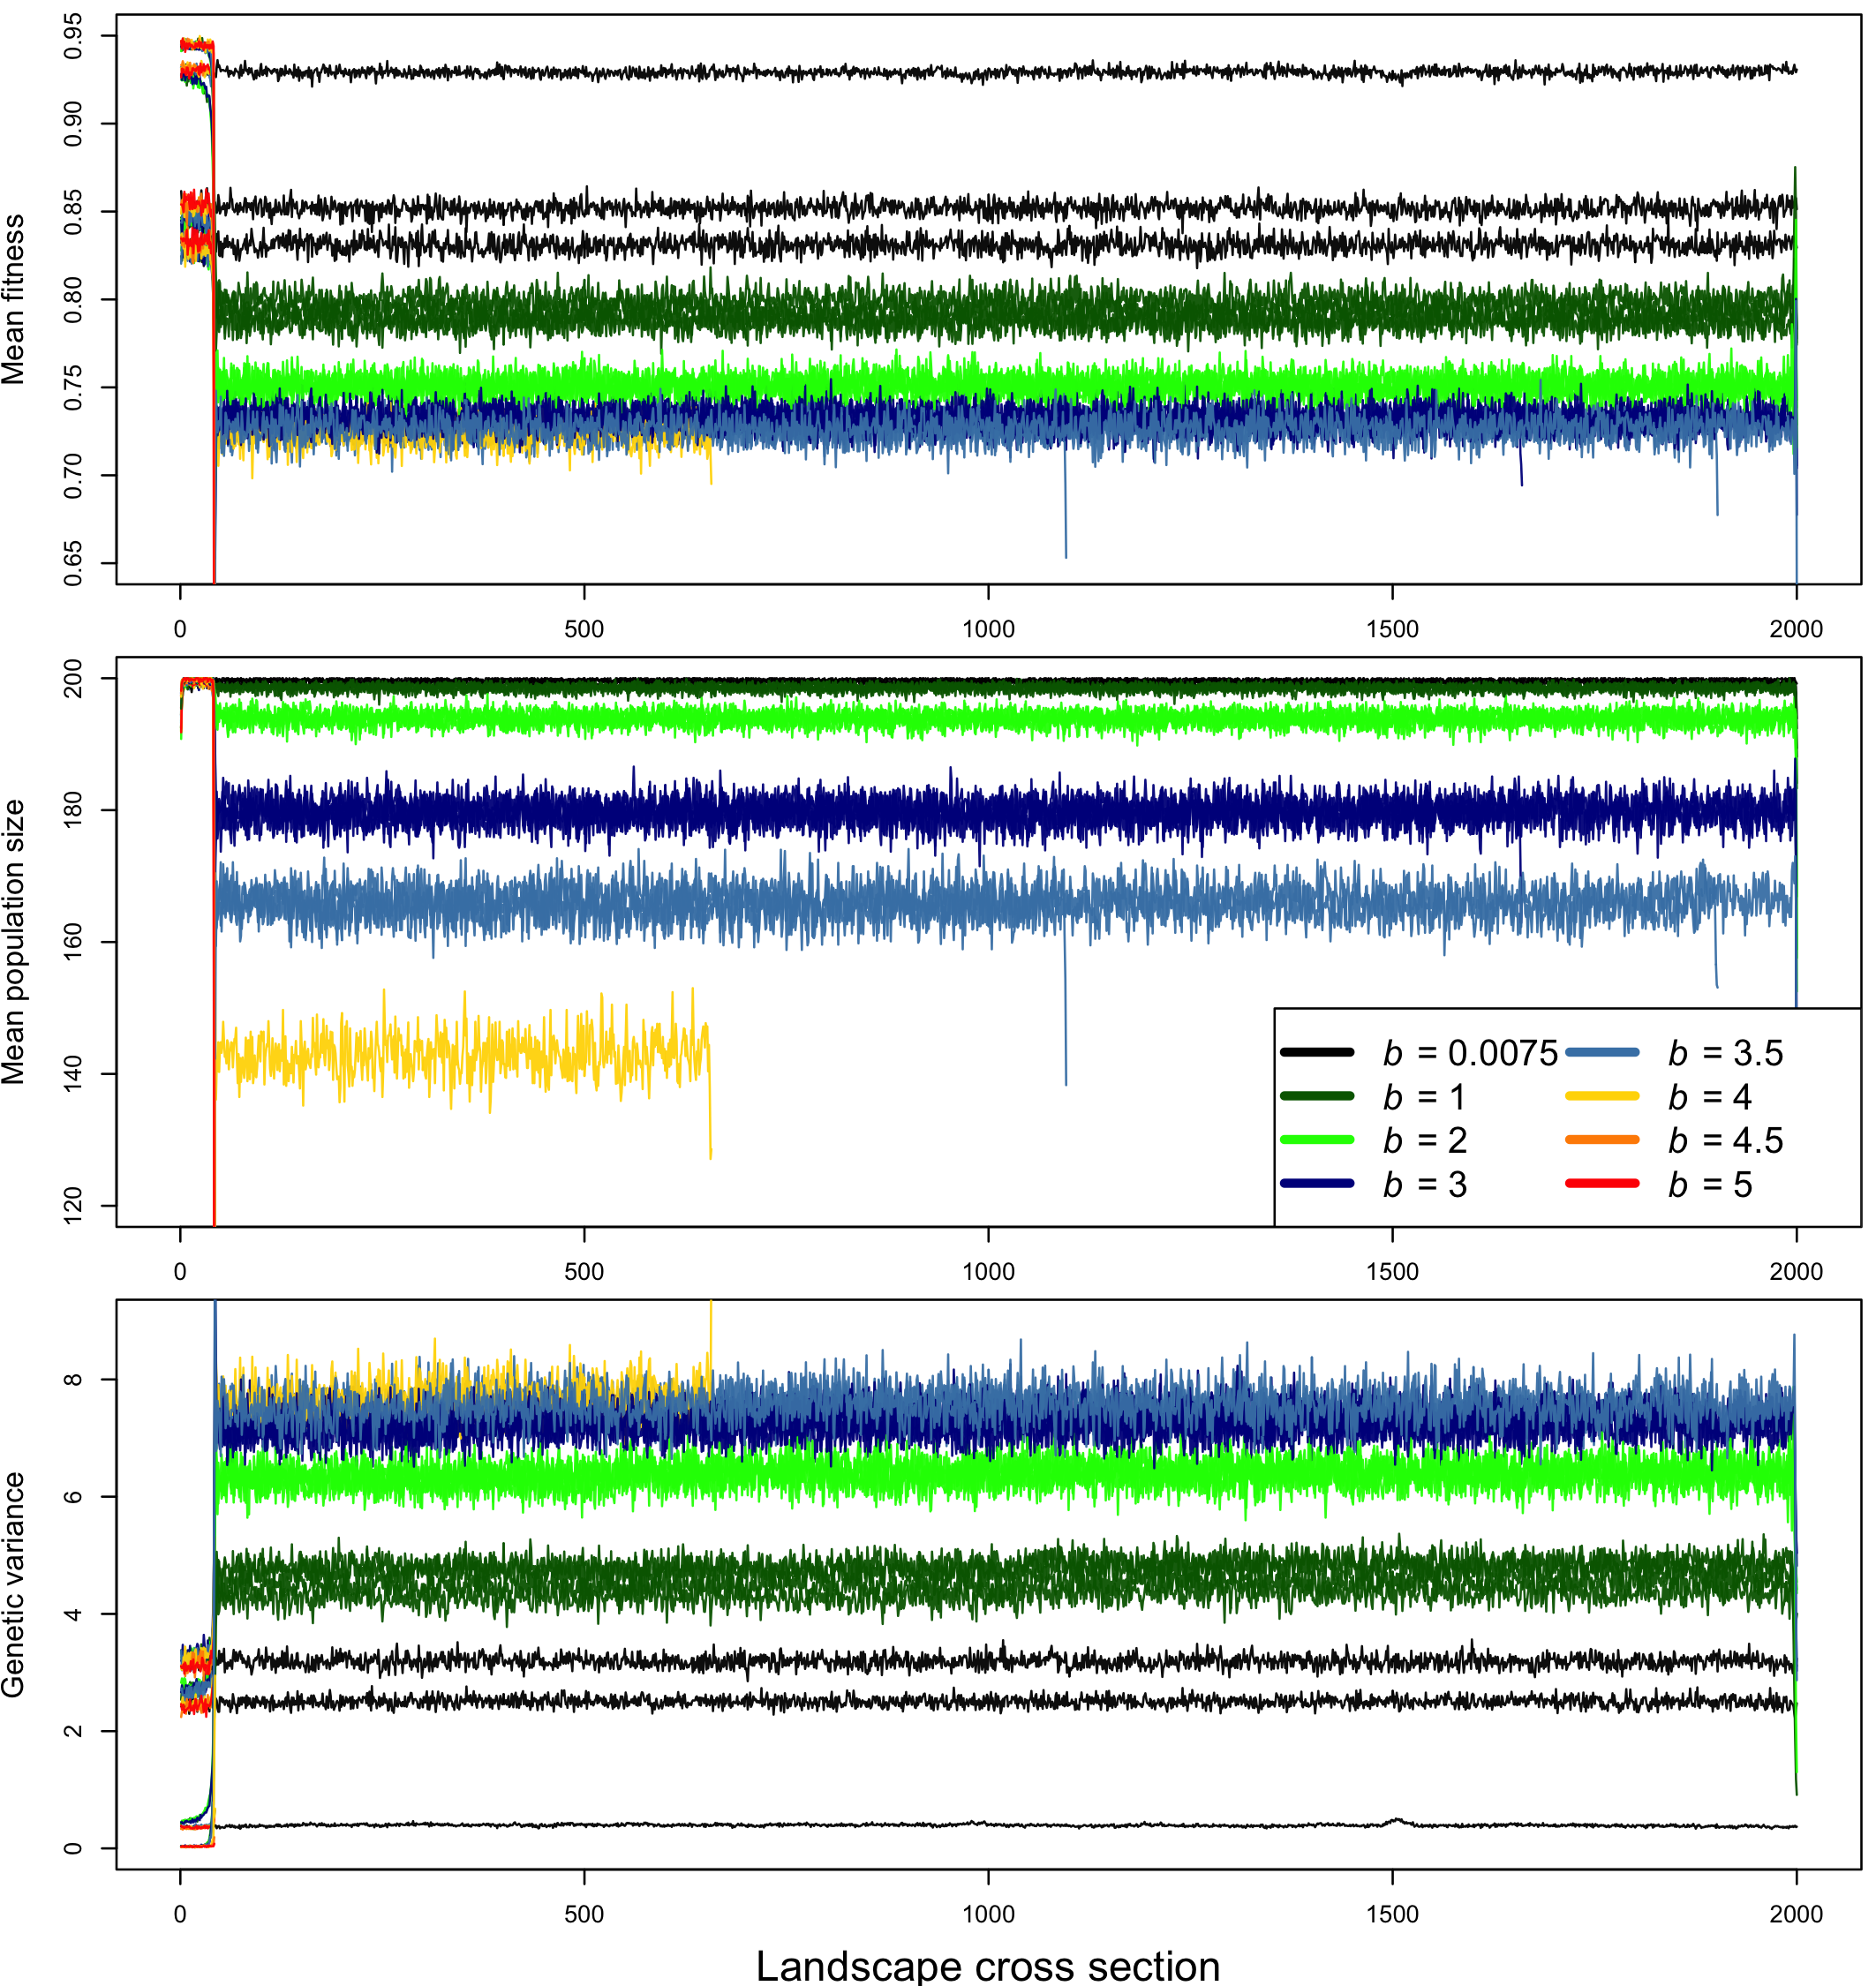
\includegraphics[width=1\linewidth]{Figures/AvgFitPopsizeGenvar_AcrossLandscape.png}}
\caption[~- Population statistics across the landscape.]{Population statistics for all genetic architecture regimes across the landscape at the end of the simulation period for all replicates. Colors match those in Figure \ref{fig:linearspeed}. Mean fitness is shown in the first panel, followed by mean population size, and then genetic variance measured within each cross section. Simulations were halted at generation 20,000 in all cases, hence slowly expanding replicates show as not having colonized the full landscape. All populations survive in the landscape core, and steeper gradients go extinct outside of this core. Within the core, each genetic architecture regime has its own equilibrium fitness and genetic variance, but once expanding over the gradient, these values are determined by the steepness of $b$, not by the genetic architecture regime. The only exception to this is for a very weak gradient, $b = 0.0075$ (black), where the different genetic architecture regimes reflect different population values across the landscape.}
\label{fig:fitness_popsize}
\end{figure}


\begin{figure}[h]
\centering
\makebox[\textwidth]{
        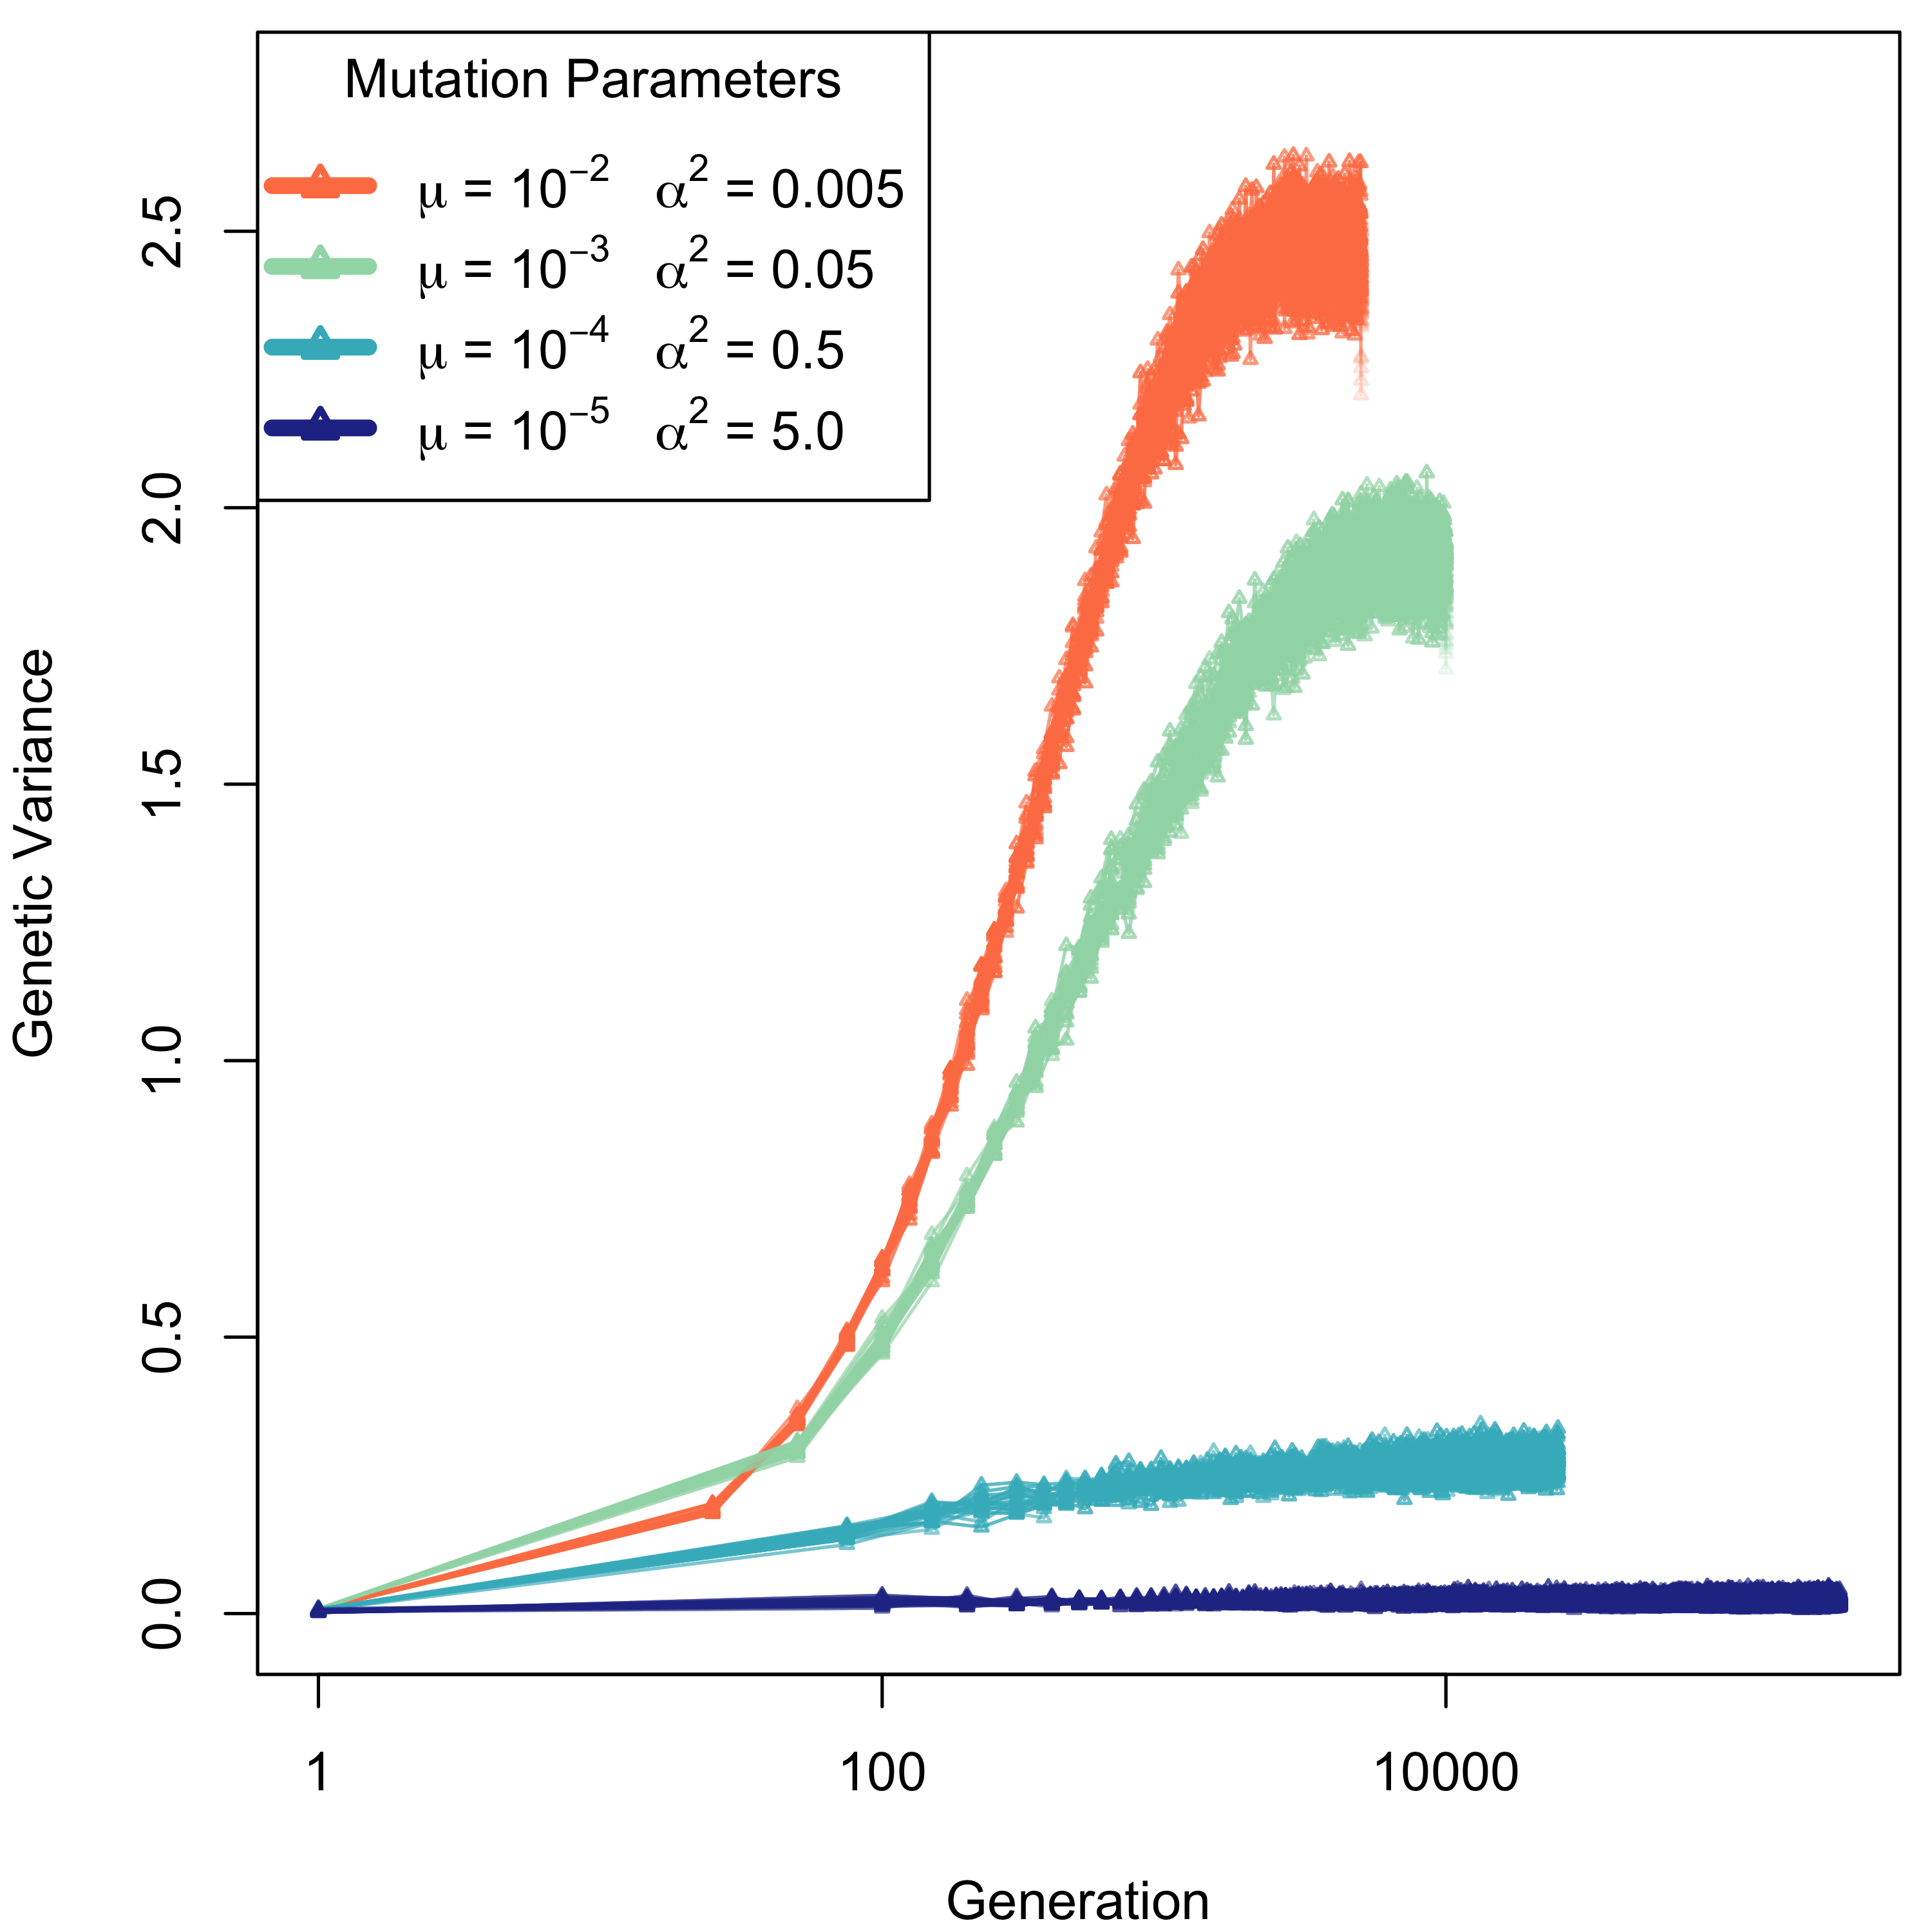
\includegraphics[width=0.9\linewidth]{Figures/CompareVa_OnePlot.png}}
\caption[~- Genetic variance across parameter sets.]{Genetic variance across parameter sets approaching respective equilibria during simulation burn-in.}
\label{fig:VaAmong}
\end{figure}


\begin{figure}[h]
\centering
\makebox[\textwidth]{
        \includegraphics[width=1\linewidth]{Figures/wait_times_200.pdf}}
\caption[~- Time spent before expansion into second patch.]{Time spent (in generations) before expansion into second patch for each genetic architecture regime with a larger dispersal kernel of $\sigma_{disperse} = 4$. Points are jittered for visualization. All points beyond the vertical dashed line are censored and did not expand during the course of the simulation.}
\label{fig:waittimes200}
\end{figure}


\begin{figure}[h]
\centering
\makebox[\textwidth]{
        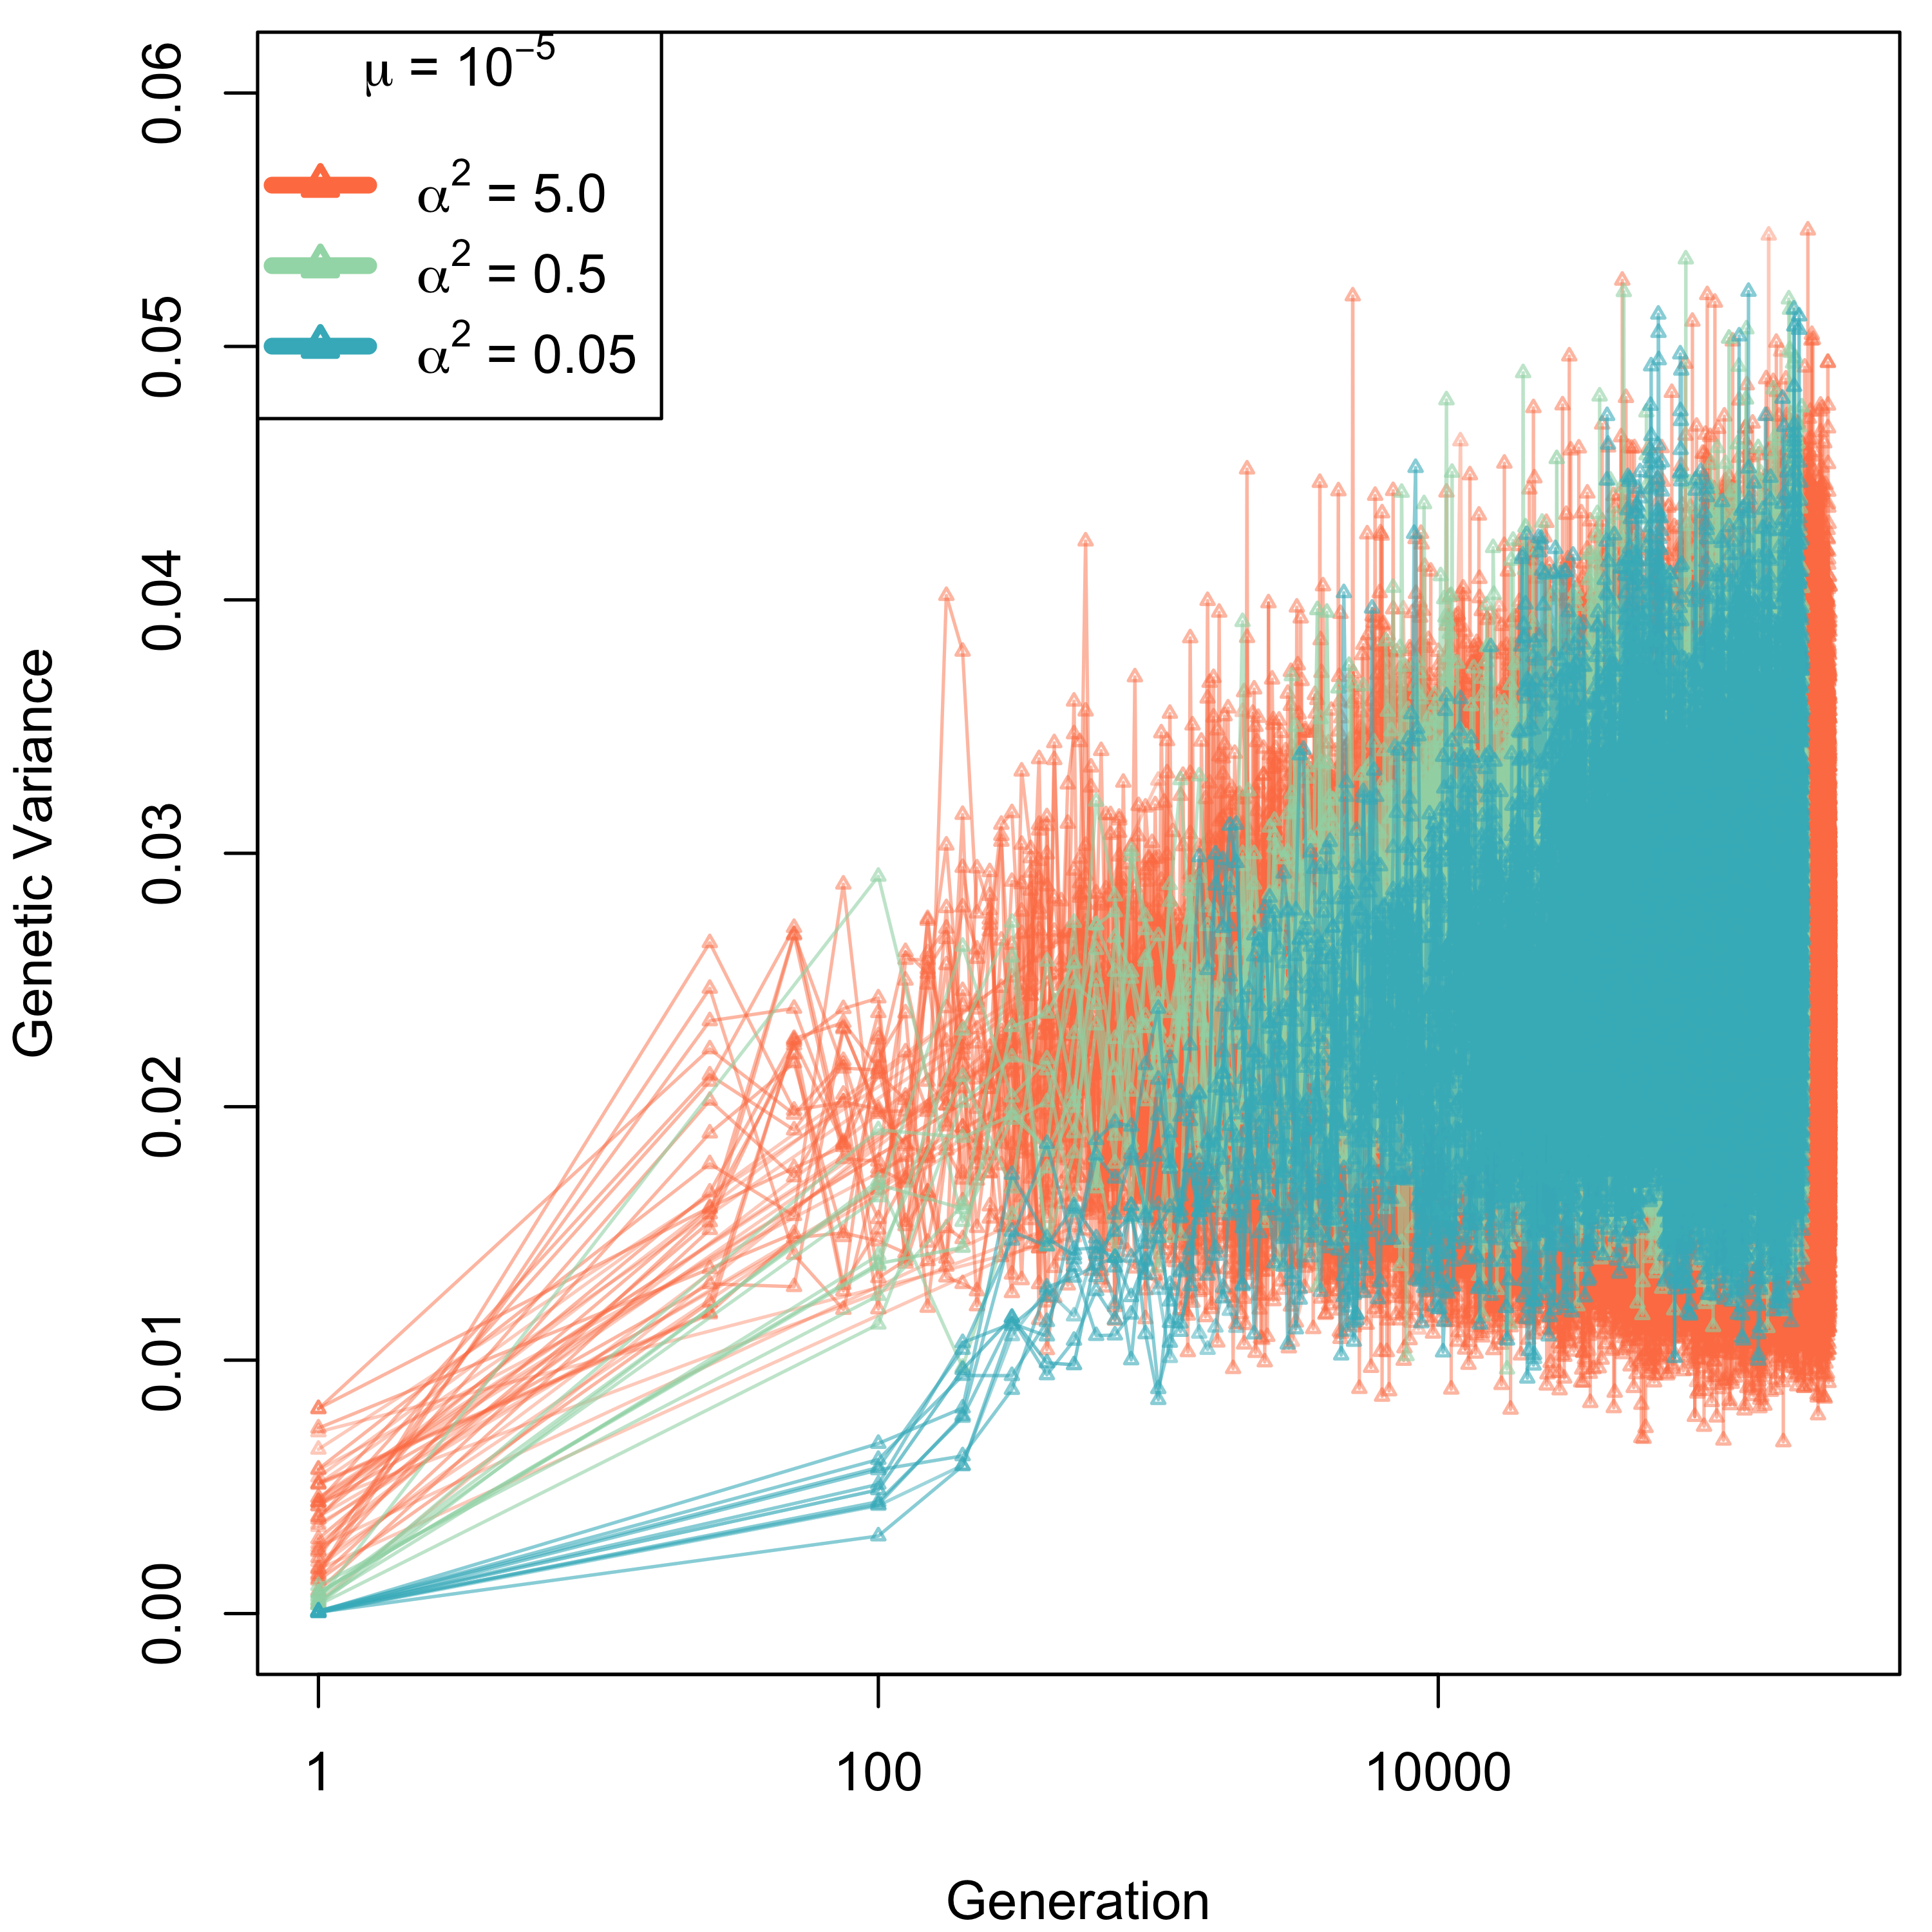
\includegraphics[width=0.9\linewidth]{Figures/constVg_CompareVa_OnePlot.png}}
\caption[~- Approximately constant genetic variance across parameter sets.]{Approximately constant genetic variance across parameter sets approaching respective equilibria during simulation burn-in.}
\label{fig:VaConst}
\end{figure}


\begin{figure}[h]
\centering
\makebox[\textwidth]{
        \includegraphics[width=0.9\linewidth]{Figures/UpdatedGrowthRatesByStep_Disp200.pdf}}
\caption[~- Mean population growth rates across patchy landscapes for large dispersal kernel.]{Mean population growth rates (number of individuals per generation) across patchy landscapes for a large dispersal kernel of $\sigma_{disperse} = 4$. $\Delta z_{opt}$ is constant at either $5$ or $10$. The size of each patch directly correlates to the number of patches on the landscape. The overall gradient increases with additional steps and can be calculated as $b = \Delta z_{opt} (number~of~patches - 1)$.}
\label{fig:disp200_multistep}
\end{figure}






